\chapter{Results}

\lettrine{A}{ll} the ideas exposed on previous chapter have been put into 
practice in order
to assess the quality of the results. The resulting piece of
software does not intend to be pretty polished and well-designed software,
neither to be very refined in terms of performance but just to be a prototype.
With this idea in mind the used language have been Python because its
easy-of-use is a good choice for rapid prototyping software.

In this chapter the quality of results are assessed and the scalability
of the tool is analyzed.

\section{Validation}\label{s:validation}

Validation consists on check out if the actual results happen to meet with what
was expected. In our case we expect the resulting pseudocode can represent the
general structure of the target application. The strategy followed for
validation will be starting with some toy examples in order to validate concrete
cases and then perform a validation in a real world application.

\subsection{Specific capabilities validation}

First step of validation is to check out the behavior of the prototype for 
the expected scenarios. The strategy is to start with toy examples and try to
increase the difficulty by adding complexity.

\subsubsection{Nesting loops}

In this test is going to be checked if subloops at different nesting levels are
well detected. The body of the most inner loop just consists on two p2p operations, the
pair ranks performs a recv while odd ranks a send. For the loops of the rest of
the levels also contains an mpi call, because if not they will be completely
invisible for us. 

One single loop detection is trivial so lets start the validation with 2 and 3 nested
loops. In figure \ref{fig:clustering_val_2} you can see the clustering performed
for the two nested loops example, meanwhile in figure
\ref{fig:clustering_val_3} there is the clustering for the three levels of
nested loops. In these figures it can be seen how there is the
same number of clusters as loops and in both cases all of them belonging to the
same phase, i.e. Explains the same amount of time of the application, what in our
model indicates that could be a hierarchical relationship between them that will
be discovered on the loops merge step. Looking on this plots, the loops merge
step is done in a bottom-right to top-left fashion.

After execute the rest of steps, the output of the first case is depicted in figure 
\ref{fig:result_val_2}. The second case output is in figure \ref{fig:result_val_3}. 

\begin{multicols}{2}
  \begin{figure}[H]
    \centering
    \includegraphics[width=0.5\textwidth]{validation/clustering_val_2}
    \caption{Clustering of validation example 1}
    \label{fig:clustering_val_2}
  \end{figure}
  \columnbreak
  \begin{figure}[H]
    \centering
    \includegraphics[width=0.5\textwidth]{validation/clustering_val_3}
    \caption{Clustering of validation example 2}
    \label{fig:clustering_val_3}
  \end{figure}
\end{multicols}

\begin{figure}[H]
    \centering
    \includegraphics[width=0.7\textwidth]{validation/result_val_2}
    \caption{Result for 2 nested loops}
    \label{fig:result_val_2}
\end{figure}
\begin{figure}[H]
    \centering
    \includegraphics[width=0.7\textwidth]{validation/result_val_3}
    \caption{Result for 3 nested loops}
    \label{fig:result_val_3}
\end{figure}

It has been demonstrated that the prototype is capable to detect an arbitrary
number of nested loops (just 3 levels have been shown here for space reasons).

\subsubsection{Phases detection}

Have been claimed that the proposed model can detect different phases of the
execution, i.e. Different loops with no hierarchical relationship that explains
different parts of the execution. In this section there is going to be validated
if it can be done in an scenario with arbitrary number of different phases having an
arbitrary nested level on every one of them. For space reasons the experiment
done is just for 3 phases, explaining different amount of time, with two nested 
levels on every phase.

In figure \ref{fig:clustering_val_4} there is the clustering for the exposed
example and in figure \ref{fig:result_val_4} the outputted pseudo-code. In the
clustering can be clearly seen the three different phases explaining 11\%, 25\%
and 42\% of the overall execution time respectively. It fits very well with we can
see on pseudocode. Taking into account that in this example every iteration
takes the same amount of time (with a certain variability), the first loop
executes $\frac{50}{350} \approx 15\%$ of the iterations, second loop 
$\frac{200}{350} \approx 57\%$ and the third $\frac{100}{350} \approx 29\%$.
Those values are strongly related with the deltas seen in the clustering. 
Additionally for every phase it can be seen two different clusters that are 
merged in the same way as explained for the ``nesting loops'' example.

With this example the multiple phases detection is demonstrated to work
correctly also together with multiple nesting loops.

\begin{figure}[H]
  \centering
  \includegraphics[width=0.5\textwidth]{validation/clustering_val_4}
  \caption{Clustering of validation example 3}
  \label{fig:clustering_val_4}
\end{figure}

\begin{figure}[H]
    \centering
    \includegraphics[width=0.7\textwidth]{validation/result_val_4}
    \caption{Result for nested loops on different phases}
    \label{fig:result_val_4}
\end{figure}

\subsubsection{Nested loops with aliasing}

The two previous tests were without taking into account the aliasing that could
appear in some cases so in order to assess the modifications introduced in
section \ref{ss:methodology_modifications} works well, some tests have been
prepared. This test consists on assess the detection of arbitrary nested
aliased loops. So there is a superloop with mpi calls, in order to detect it,
with some aliased subloops in its body. For space reasons, two examples are
done with two and three nested aliased loops respectively.

\begin{multicols}{3}
  \begin{figure}[H]
    \centering
    \includegraphics[width=0.3\textwidth]{validation/clustering_val_5}
    \caption{Clustering for 2 nested aliased loops}
    \label{fig:clustering_val_5}
  \end{figure}
  \columnbreak
  \begin{figure}[H]
    \centering
    \includegraphics[width=0.3\textwidth]{validation/clustering_val_6}
    \caption{Clustering of 3 nested aliased loops}
    \label{fig:clustering_val_6}
  \end{figure}
  \columnbreak
  \begin{figure}[H]
    \centering
    \includegraphics[width=0.3\textwidth]{validation/clustering_val_7}
    \caption{Clustering of 3 nested aliased loops with hidden superloop}
    \label{fig:clustering_val_7}
  \end{figure}
\end{multicols}

\begin{figure}[H]
    \centering
    \includegraphics[width=0.7\textwidth]{validation/result_val_5}
    \caption{Result for 2 nested aliased loops}
    \label{fig:result_val_5}
\end{figure}
\begin{figure}[H]
    \centering
    \includegraphics[width=0.7\textwidth]{validation/result_val_6}
    \caption{Result for 3 nested aliased loops}
    \label{fig:result_val_6}
\end{figure}
\begin{figure}[H]
    \centering
    \includegraphics[width=0.7\textwidth]{validation/result_val_7}
    \caption{Result for 2 nested aliased loops with hidden superloop}
    \label{fig:result_val_7}
\end{figure}

If you look at the clustering you will see how just two clusters appears in both
cases. The top-left cluster is representing the outer loop meanwhile the bottom-right
represents both inner loops (figure \ref{fig:clustering_val_5}) in first example 
and all three for the second (figure \ref{fig:clustering_val_6}), here is where 
the aliasing appears. For detecting the multiple aliased loops the technique
described in \ref{ss:cluster_aliasing} is applied and the results are
satisfactory as you can see on outputted pseudo-codes \ref{fig:result_val_5} and
\ref{fig:result_val_6}.

Additionally has been tested the ``hidden superloop'' detection just by
removing the \texttt{MPI\_Barrier} in line 17. It will cause the top-left
cluster representing the outer loop disappear as you can see on clustering in
figure \ref{fig:clustering_val_7} and the results on figure
\ref{fig:result_val_7}. This superloop have been detected because the
additional modifications introduced in section \ref{ss:hidden_superloop_det}.

\subsubsection{Data conditions}

Last thing to check out is whether the model can detect loops with some mpi calls
under data conditions. This scenario was introduced in section
\ref{ss:cluster_split} where also the modifications introduced to the model are
explained. Could happen that some communications are executed just for some set
of iterations, for example in order to save communications overhead. In this
last test two examples are done. 

First of them will show how in some situations
even if there an mpi call under a data condition, the model can solve it without
the extra checks introduced in \ref{ss:cluster_split} building up a valid
representation of the applications' structure. It will consist on a mpi call at
the beginning of the loop body that is executed just in odd iterations, then
after that a typical send for odd ranks and recv for pair ranks is executed. The
results can be seen in figure \ref{fig:result_val_8}. Even if the original code
was one single loop of 100 iterations with the \texttt{MPI\_Barrier} being
executed just for odd iterations, the representation outputted by the model is 
one outer loop of 50 iterations and one inner loop of 2 iterations. This is
completely valid representation that can be seen if we compare the dynamic
aspect of both the original and the outputted loop. 

\begin{figure}[H]
    \centering
    \includegraphics[width=0.7\textwidth]{validation/result_val_8}
    \caption{Result for mpi call under data condition 1}
    \label{fig:result_val_8}
\end{figure}

Second example is about when the extra check mechanism must act. It shares
about the same structure of the first example but with additional communications
executed before the conditioned mpi call. The key point is that now the
conditioned call is surrounded by non conditioned calls. You can see the result
for this second example on figure \ref{fig:result_val_9}. Since we do not have
information about to with what data the execution of a given mpi call is
conditioned, the way to depict a given call is being executed under a data
condition is by means of what it can be seen in line 24 of the result. It
represents the probability to be executed. Have the knowledge about in what
iterations are these kind of mpi calls executed could be a big deal so future
developments in this sense have to be done.

\begin{figure}[H]
    \centering
    \includegraphics[width=0.7\textwidth]{validation/result_val_9}
    \caption{Result for mpi call under data condition 2}
    \label{fig:result_val_9}
\end{figure}

\subsection{Real application validation}

The proposal explained in this thesis is devoted to deal with real world
applications so the last step of validation is to assess the correctness of the
analysis for them. For time reasons just one application has been analyzed
for medium size execution.

There are two ways to assess the quality of the results in this case:
\begin{enumerate}[label=\roman*)]
  \item Inspecting manually the source code of the application looking for the
    general structure. 
  \item Using Paraver visualizer. With paraver it can be analyzed where and when
    every mpi call has taken place and the order of them. 
%  \item Do it automatically. Remember that we have developed a mechanism for
%    label the mpi calls with loop id where they belongs. The validation will
%    consists on check out if all mpi calls in same cluster have the same label.
\end{enumerate}

The first presents to be very tough and error prone when dealing with
huge source codes so it is discarded. Using paraver is a good alternative since
the general structure can be easily visualized and for sure the performance
information. 

\subsubsection{Lulesh 2.0}

Lulesh is understood as ``Livermore Unstructured Lagrangian Explicit
Shock Hydrodynamics''. It approximates the hydrodynamics equations discretely 
by partitioning the spatial problem domain into a collection of volumetric 
elements defined by a mesh\footnote{https://codesign.llnl.gov/lulesh.php}.

The execution have been done with 128 mpi ranks and for 30 iterations. On figure
\ref{fig:clustering_val_10} you can see the clustering. It seems a quite simple
application since just appears one cluster. It would mean that there is just one
loop with no nesting loops. 
In figure \ref{fig:result_val_10} there is the outputted pseudocode.
For space reasons, this code have been previously filter in order to only show
the structure for rank 0. Since Lulesh is a SPMD program we can expect the
pseudo-code for all the 128 ranks to be quite similar so only the presented one
will be validated. Additionally the threshold on computation phases have been
set on 6ms.

\begin{figure}
  \centering
  \includegraphics[width=0.5\textwidth]{validation/clustering_val_10}
  \caption{Clustering of lulesh 2.0 128 ranks 30 iterations}
  \label{fig:clustering_val_10}
\end{figure}

\begin{figure}
    \centering
    \includegraphics[width=\textwidth]{validation/result_val_10}
    \caption{Intern structure of lulesh 2.0 - Rank 0 - Computation threshold 6ms}
    \label{fig:result_val_10}
\end{figure}

First thing to take into account is that this is a single
loop with no nested loops that executes 30 iterations. This first part is quite
easy to check out looking to the trace that corresponds to this execution on
figure \ref{fig:lulesh_trace_1}. It can be easily identified an structure that
is being repeated during the whole execution. Even if it is a bit tricky it can
be counted that there are 30 repetitions.
If now we enter to the body of the loop the first think it can be seen is that
there is an \texttt{MPI\_Allreduce} on the communicator 1 that is executed the
96,6\% of the times that corresponds to 29 iterations what is validated in
figure \ref{fig:lulesh_trace_2} (this table contains the mpi call counts for the
body of the execution, cutting initialization and finalization). About the rest 
of the mpi calls also can be
validated with the same table by counting the times that appears on the
pseudo-code and multiply it by the number of iterations. It is demonstrated how
the mpi calls count is related perfectly with what can be seen on trace.
\begin{enumerate}[label=\roman*)]
  \item \texttt{MPI\_Comm\_rank} $9*30=270$
  \item \texttt{MPI\_Comm\_rank} $17*30=510$
  \item \texttt{MPI\_Comm\_rank} $10*30=300$
  \item \texttt{MPI\_Comm\_rank} $3*30=90$
  \item \texttt{MPI\_Comm\_rank} $17*30=510$
\end{enumerate}

\begin{figure}
    \centering
    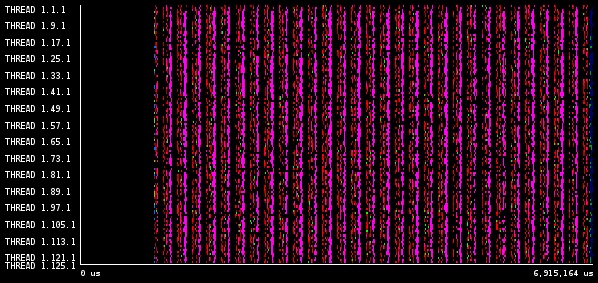
\includegraphics[width=0.7\textwidth]{validation/lulesh_trace_1}
    \caption{Lulesh2.0 128 mpi ranks - 30 iterations trace}
    \label{fig:lulesh_trace_1}
\end{figure}

\begin{figure}
    \centering
    \includegraphics[width=0.7\textwidth]{validation/lulesh_trace_2}
    \caption{Lules2.0 mpi call count for rank 0}
    \label{fig:lulesh_trace_2}
\end{figure}


We already have seen how, at least, the number of times every mpi call is
executed corresponds with the actual execution, now we need to figure out if the
presented structure of the body of the loop is correct. To do so we can compare
the different big computational phases that appears both in pseudocode and in
trace. For this purpose in figure \ref{fig:lulesh_trace_3} it can be seen a 
detailed view for a given iteration. The times for the different phases have
been taken from the rank 0 even if in trace there are shown all ranks. This is
because by this way is much easier to visualize the structure of the iteration. There
are five long computational phases and if we perform a comparison between the
computational phases detected by our tool and the phases on trace we
can realize they are the same and in the same order so have been demonstrated
the structure detected is correct. We can perform the same comparison for the
IPC with same result. Additionally for assess the mpi calls are
correctly arranged between these computational phases, the figure
\ref{fig:lulesh_trace_4} can be consulted. Here the mpi call count have been
divided into 5 parts that corresponds to the splits that the different big
computational phases does. 

\begin{figure}
    \centering
    \includegraphics[width=0.7\textwidth]{validation/lulesh_trace_3}
    \caption{Lules2.0 detailed view for a single iteration}
    \label{fig:lulesh_trace_3}
\end{figure}
\begin{figure}
    \centering
    \includegraphics[width=0.5\textwidth]{validation/lulesh_trace_4}
    \caption{Lules2.0 mpi call count for a single iteration splited by
    computational phases}
    \label{fig:lulesh_trace_4}
\end{figure}

By analyzing the trace have been demonstrated how the developed tool can
satisfactorily detect the internal structure of a well-known real application,
in this case, Lulesh.


\section{Scalability}\label{s:scalability}

One of the motivations for this work is to be scalable or at least more scalable
than the current state of the art. In this section we have driven a little analysis
about scalability. 

As has been explained previously, the key point of the proposal done in this
thesis is the clustering step (section \ref{ss:loops_clustering}) that is feed
by a reduction of the input trace (section \ref{ss:trace_reduction}). This
reduction is the most important point for the scalability of the proposal. What
is understood as scalability is that the method does not degrade, or degrade
moderately in terms of required resources when the input data grows
dramatically. We have argued that since the HPC applications used to be very
repetitive, the number of mpi calls to clusterize will remain almost constant
despite the size of the execution. 

In order to assess our assumptions, a quantitative analysis have been done by
executing NPB benchmarks for A,B and C classes and for 8, 16 and 32 ranks (9,16
and 36 for special cases of BT and SP that restrict the number of ranks to
squared values, i.e. $1^{2}, 2^{2}, 3^{2}, \cdots$). For every execution first
step of the proposed methodology have been executed, i.e. Reduction step and
the number of unique mpi calls have been calculated, remember we consider two
same call path calls to be different if they have been performed by different
processes. This information is plotted
in figure \ref{fig:scalability_results}. For every benchmark you can see a
matrix where columns are the size of the problem and rows number of processes, the
colors indicates the relative quantity of mpi calls, being the darker the
greater (for see the numbers go to \ref{s:nunique_mpi_calls}) . 

By a quick peek it can be seen the number of mpi calls remains despite the
growing size of the execution time, so the assumption about repetitivity has 
been demonstrated. On the other axis the trend is quite different since there is
an increment on mpi calls number. This phenomena is obvious since we are not
merging calls from different processes on first step, so at least they are
incrementing with the same factor as the increment of the number of processes.

\begin{figure}
    \centering
    \begin{subfigure}[b]{0.3\textwidth}
        \includegraphics[width=\textwidth]{scalability/cg_plot_heatmap.png}
        \caption{CG}
        \label{fig:cg_sca}
    \end{subfigure}
    \quad
    \begin{subfigure}[b]{0.3\textwidth}
        \includegraphics[width=\textwidth]{scalability/ft_plot_heatmap.png}
        \caption{FT}
        \label{fig:ft_sca}
    \end{subfigure}
    \quad   
    \begin{subfigure}[b]{0.3\textwidth}
        \includegraphics[width=\textwidth]{scalability/lu_plot_heatmap.png}
        \caption{LU}
        \label{fig:lu_sca}
    \end{subfigure}
    
    \begin{subfigure}[b]{0.3\textwidth}
        \includegraphics[width=\textwidth]{scalability/mg_plot_heatmap.png}
        \caption{MG}
        \label{fig:mg_sca}
    \end{subfigure}
    \quad
    \begin{subfigure}[b]{0.3\textwidth}
        \includegraphics[width=\textwidth]{scalability/is_plot_heatmap.png}
        \caption{IS}
        \label{fig:is_sca}
    \end{subfigure}
    \quad
    \begin{subfigure}[b]{0.3\textwidth}
        \includegraphics[width=\textwidth]{scalability/ep_plot_heatmap.png}
        \caption{EP}
        \label{fig:ep_sca}
    \end{subfigure}
    
    \begin{subfigure}[b]{0.3\textwidth}
        \includegraphics[width=\textwidth]{scalability/sp_plot_heatmap.png}
        \caption{SP}
        \label{fig:sp_sca}
    \end{subfigure}
    \quad
    \begin{subfigure}[b]{0.3\textwidth}
        \includegraphics[width=\textwidth]{scalability/bt_plot_heatmap.png}
        \caption{BT}
        \label{fig:bt_sca}
    \end{subfigure}
    \quad
    \caption{Number of unique mpi calls}
    \label{fig:scalability_results}
\end{figure}

To check out how the proposed tool is scaling with growing number of processes
and growing input, several executions with two different NPB applications have
been done. The applications are CG and MG. The interest in these two
applications resides in the fact that CG have less unique mpi calls but more
repeated and MG have much more unique mpi calls but less repeated. You can see 
the results on images \ref{fig:scalability_results_cg} for CG and 
\ref{fig:scalability_results_mg} for MG (the numbers can be seen on section
\ref{s:strdect_exec_times}. 

In both cases can be seen how the overall execution time is highly dominated
by the Reduction phase being the responsible for about the 100\% of the time for
CG (figure \ref{fig:cg_stdrec_rel}) and about 90\% of the time for the analysis
of MG traces (figure \ref{fig:mg_stdrec_rel}). 
About strong scaling, i.e. When the number of processes are being
increased but the size of the problem remains the same, it can be seen
how time grows linearly with number of ranks in MG
(figure \ref{fig:mg_strdec_abs}) but seems to grow faster in case of CG (figure
\ref{fig:cg_strdec_abs}). As can be seen on first table in section \ref{s:nunique_mpi_calls} the
number of mpi calls are just doubling every time scaling on ranks so this is not
the reason for this super-linear growth. 
When scaling the problem size, the execution time of the
structure detector grows slowly, it can be said in a logarithmic fashion. 

The fundamental reason that explains the Reduction phase times is the size of
the input traces as can be seen on \ref{fig:trace_sizes} so as has been
introduced in previous chapters, the reduction phase complexity is linear with 
trace size.

Additionally can be seen how the merge step is much bigger in case of MG than in
CG, the reason is that MG has much more nested loops but the manly reason is
that since reduction phase is much smaller, the relative weight of the rest of
the phases is bigger.

\begin{figure}
    \centering
    \begin{subfigure}[b]{0.45\textwidth}
        \includegraphics[width=\textwidth]{scalability/strdect_cg_absolute_times.png}
        \caption{Stacked absolute times}
        \label{fig:cg_strdec_abs}
    \end{subfigure}
    \medspace
    \begin{subfigure}[b]{0.45\textwidth}
        \includegraphics[width=\textwidth]{scalability/strdect_cg_rel_times.png}
        \caption{Stacked relative times}
        \label{fig:cg_stdrec_rel}
    \end{subfigure}
    \caption{Structure detection times for CG application}
    \label{fig:scalability_results_cg}
\end{figure}

\begin{figure}
    \centering
    \begin{subfigure}[b]{0.45\textwidth}
        \includegraphics[width=\textwidth]{scalability/strdect_mg_absolute_times.png}
        \caption{Stacked absolute times}
        \label{fig:mg_strdec_abs}
    \end{subfigure}
    \medspace
    \begin{subfigure}[b]{0.45\textwidth}
        \includegraphics[width=\textwidth]{scalability/strdect_mg_rel_times.png}
        \caption{Stacked relative times}
        \label{fig:mg_stdrec_rel}
    \end{subfigure}
    \caption{Structure detection times for MG application}
    \label{fig:scalability_results_mg}
\end{figure}

\begin{figure}
    \centering
    \begin{subfigure}[b]{0.45\textwidth}
        \includegraphics[width=\textwidth]{scalability/mg_tracesize.png}
        \caption{MG Trace sizes}
        \label{fig:mg_trace_size}
    \end{subfigure}
    \medspace
    \begin{subfigure}[b]{0.45\textwidth}
        \includegraphics[width=\textwidth]{scalability/cg_tracesize.png}
        \caption{CG Trace size}
        \label{fig:cg_trace_size}
    \end{subfigure}
    \caption{Trace sizes}
    \label{fig:trace_sizes}
\end{figure}
